\section{Crawling\label{crawling}}
In order to crawl large numbers of web pages fast, a
distributed system of crawlers was set up, along with
automation scripts written in {\tt BASH}. The scripts allowed
machines and processes to be added to the pool of `crawlers'.  Files
were shuttled to a master machine using {\tt rsync} periodically,
and various cleanup scripts were used in order to ensure that crawler
instances retained a certain level of available disk space.  This
approach was inspired by the distributed crawling method outlined by
\citeA{page1998}.

One difference is that
\nr{} relies heavily on Redis, whereas \citeauthor{page1998} write
about a custom {\it URL server} that was supposedly built from scratch.
Another key difference is
the method of distributing and storing files.  Rather than some
distributed, fault-tolerant filesystem, \nr{} simply stores all the
compressed web pages on a RAID-1 file system.  This design
choice was made for three reasons.  Firstly, the task of this
project is limited to recent news, so not as much disk storage is
needed, as compared to a tool for the general web.  Secondly,
disk space has advanced a lot since Google was launched;
renting a dedicated server with 4TB of disk space now costs
as low as €33 a month\footnote{Price estimated from Hetzner's server auction \url{https://www.hetzner.com/sb}, 2020}.  Lastly, setting up a distributed filesystem
is costly, requires time, specialised expertise, and ties the
project to `the cloud', effectively ruling out the possibility of
development and usage without an internet connection.
Relying on an
old-fashioned single hard drive allowed \nr{} to be developed fast,
and at times without a connection to the internet.

\begin{figure}
    \centering
    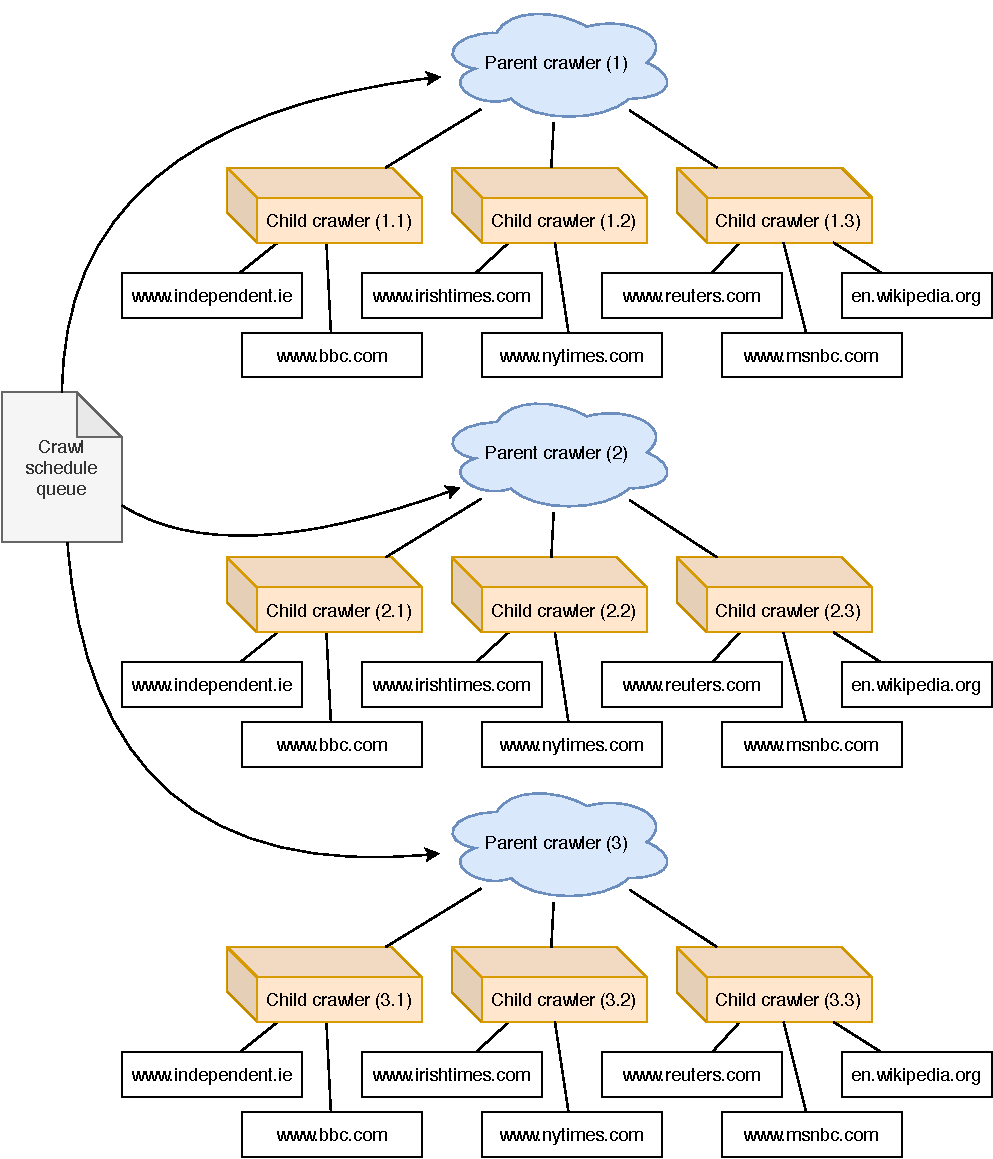
\includegraphics[width=0.95\textwidth]{media/crawler.pdf}
    \caption{
        A closer look at the distributed crawler from
        Figure \ref{overview-fig}.
    }
\end{figure}